\chapter{SCRR Supplementary Material} \label{chap:appendix-scrr}


\section{Self-Clocked Round-Robin Scheduling}
\label{app:algs}

\begin{algorithm}[b!]
\caption{SCRR-basic Enqueue}
\label{alg:scrr-basic-enq}
\begin{algorithmic}
\Function{Enqueue}{pkt}

\Call{$cur\_queue \gets classify$}{pkt}
\If{$cur\_queue$ is inactive}
% \State $a = 1$
\State $sub\_queues.tail \gets cur\_queue$
\State $rounds \gets rounds + 1$
\EndIf
\State $pkt.virtual \gets max(virtual\_clock, cur\_queue.clock)$
\State $cur\_queue.clock \gets pkt.virt\_tag + pkt.length$
\State
\Call{$cur\_queue.enqueue$}{pkt}
\EndFunction
\end{algorithmic}
\end{algorithm}

\begin{algorithm}[b!]
\caption{SCRR-basic Dequeue}
\label{alg:scrr-basic-deq}
\begin{algorithmic}
\Require $NP \ge 0$
\Comment{Packet count}
\Function{Dequeue}{}
\Comment{Packet Retrieval}
\If{$NP == 0$}
\Return NULL
\EndIf
\State $cur\_queue \gets sub\_queues.head$
\State $pkt \gets cur\_queue.dequeue()$
\State $NP \gets NP - 1$

\Comment{Global Clock Advance}
\If{$NP == 0$}
\State $virtual\_dequeue \gets pkt.virtual + pkt.length$
\State $virtual\_clock \gets virtual\_dequeue$
\ElsIf{$pkt.virtual > virtual\_dequeue$}
\State $virtual\_dequeue \gets pkt.virtual$
\EndIf

\Comment{Sub-Queue Round Robin}
\State $virtual\_next \gets pkt.virtual\_time + pkt.length$
\If{$virtual\_next > virtual\_clock$ or $cur\_queue$ is empty}
\If{$rounds \leq 0$}
\State $virtual\_clock \gets virtual\_dequeue$
\State $rounds \gets all\_queues.length$
\EndIf
\State $rounds \gets rounds - 1$
\State $sub\_queues.head \gets cur\_queue.next$
\If{$cur\_queue$ is not empty}
\State $sub\_queues.tail \gets cur\_queue$
\EndIf
\EndIf

\Return $pkt$
%     \State $X \gets X \times X$
%     \State $N \gets \frac{N}{2}$  \Comment{This is a comment}
% \ElsIf{$N$ is odd}
%     \State $y \gets y \times X$
%     \State $N \gets N - 1$
% \EndIf
\EndFunction
\end{algorithmic}
\end{algorithm}


This section expands on the design of the Self-Clocked
Round-Robin (SCRR) packet scheduler. Both \textit{SCRR-basic} and
\textit{SCRR} with its enhancements are presented.

\subsection{Pseudo code of SCRR-basic}
\label{app:algs-basic}

SCRR-basic is the simplest of all the variants of SCRR.
% , and the one
% most similar to \textit{SCFQ} and \textit{STFQ}.
The pseudo-code for the \textbf{enqueue process} of SCRR-basic is
shown in Algorithm \ref{alg:scrr-basic-enq}. This is the process that
is run when a new packet arrives at the scheduler. First, the arrived
packet passes through the classifier to obtain its sub-queue handle,
i.e. the sub-queue where it will be enqueued. When doing per-flow
classification, the 5-tuple from the packet header is used to select
a sub-queue (source IP, destination IP, protocol, source transport
port and destination transport port). Other QoS classifiers can also be used
with SCRR. The current sub-queue may be active (already in the
schedule) or inactive (empty). In the case the sub-queue is inactive,
it is added at the end of the schedule, the schedule is a simple
linked list of sub-queues. Tagging a packet with its virtual time is implementation dependant and usually done in the metadata associated with the packet. The packet virtual time is computed here
exactly like \textit{STFQ} \cite{stfq}, i.e., the most recent of the
global clock and the finish time of the previous packet added to the
sub-queue. The virtual time of the sub-queue is updated with the
finish time of the new packet by adding its length in bytes. In the
weighted version of SCRR, the packet length would be multiplied by the
sub-queue weight. Ultimately, the packet is added to the SKB list of
the corresponding sub-queue.

The pseudo-code for the \textbf{dequeue process} of SCRR-basic is shown in Algorithm \ref{alg:scrr-basic-deq}. This is the process that is run when a packet needs to be sent over the outgoing link. First,
a packet is extracted from the current sub-queue. Then, the global
clock advance is computed. While conceptually similar to \textit{STFQ}
\cite{stfq},  SCRR makes sure that the clock
can only go forward. Then, to advance the global clock, the
scheduler maintains a temporary \textit{virtual\_dequeue} clock that
tracks the largest virtual time of packets dequeued during the
scheduling round. After finishing a scheduling round, the global
clock is set to \textit{virtual\_dequeue}. The next part is where SCRR distinguishes itself from \textit{STFQ}. SCRR uses the virtual time of
the next packet in the sub-queue to decide if it stays on that
sub-queue or round robin to the next sub-queue. If the virtual time is
in the future (greater than current clock), or if the sub-queue is
empty, then the scheduler moves on to the next sub-queue (that will be
used next time the function is called). If a number of scheduling
rounds equal to the number of sub-queues has elapsed, the virtual
clock is updated with \textit{virtual\_dequeue} (the largest of the
packet virtual times dequeued during that scheduling round). If the
sub-queue is not empty, it is put at the back of the schedule, so that
its packets can be sent at the next scheduling round.

The dequeue process must properly keep track of scheduling rounds. The
enqueue process may add a previously inactive sub-queue to the current
scheduling round. Tracking the scheduling round is needed to ensure
that the global clock is only updated between rounds. If the global
clock were to be updated after each packet transmission, the later
sub-queues might fall further behind the global clock, leading to
large unwanted packet bursts.

The algorithm describes SCRR-basic using the \textit{start-time} of
the packet like STFQ \cite{stfq}. SCRR can also be implemented using
the \textit{finish-time} of the packet, similar to SCFQ \cite{scfq}. We
chose the \textit{start-time} because it enables
us to make SCRR's implementation simpler by computing the virtual time
of the next packet without any information about that packet.

\begin{algorithm}[t!]
\caption{SCRR Enqueue (with enhancements)}
\label{alg:scrr-neia-enq}
\begin{algorithmic}
\Function{Enqueue}{pkt}
\State
\Call{$cur\_queue \gets classify$}{pkt}
\If{$cur\_queue$ is inactive}

\Comment{No Empty}
\If{$cur\_queue.clock <= virtual\_clock$ or $nq$ == 0}
\Comment{Sparse Flow Optimization}
\State $new\_queues.tail \gets cur\_queue$
\State $rounds \gets rounds + 1$
\Else
\State $old\_queues.tail \gets cur\_queue$
\EndIf
\EndIf
\State
\Call{$cur\_queue.enqueue$}{pkt}
\EndFunction
\end{algorithmic}
\end{algorithm}

\begin{algorithm}[th!]
\caption{SCRR Dequeue (with enhancements)}
\label{alg:scrr-neia-deq}
\begin{algorithmic}
\Require $NP \ge 0$
\Comment{Packet count}
\Require $nq \ge 0$
\Comment{Active sub-queue count}
\Function{Dequeue}{}
\Comment{Packet Retrieval}

\If{$NP == 0$}
\Return NULL
\EndIf

\Comment{Sparse Flow Optimization}
\State $cur\_queue \gets new\_queues.head()$
\If{$cur\_queue$ is null}
\State $cur\_queue \gets old\_queues.head()$
\EndIf
\State $pkt \gets cur\_queue.dequeue()$
\State $NP \gets NP - 1$

\Comment{No Packet Metadata}
\If{$cur\_queue.clock < virtual\_previous$}
\If{$config.initial\_advance$}
\Comment{Initial Advance}
\State $virtual\_pkt \gets virtual\_previous + pkt.length$
\Else
\State $virtual\_pkt \gets virtual\_clock$
\EndIf
\Else
\State $virtual\_pkt \gets cur\_queue.clock$
\EndIf
\State $virtual\_next \gets virtual\_pkt + pkt.length$
\State $cur\_queue.clock \gets virtual\_next$

\Comment{Global Clock Advance}

\If{$NP == 0$}
\State $virtual\_dequeue \gets pkt.virtual + pkt.length$
\State $virtual\_previous \gets virtual\_clock$
\State $virtual\_clock \gets virtual\_dequeue$
\ElsIf{$pkt.virtual > virtual\_dequeue$}
\State $virtual\_dequeue \gets pkt.virtual$
\EndIf

\Comment{Sub-queue Round Robin}
\If{$virtual\_next > virtual\_clock$ or $cur\_queue$ is empty}
\If{$rounds  \leq 0$}
\State $virtual\_previous \gets virtual\_clock$
\State $virtual\_clock \gets virtual\_dequeue$
\State $rounds \gets nq$
\EndIf
\State $rounds \gets rounds - 1$
\State $rr\_queue \gets rr\_queue.next$
\If{$cur\_queue$ is not empty}
\State $old\_queues.tail \gets cur\_queue$
\EndIf
\EndIf

\Return $pkt$
%     \State $X \gets X \times X$
%     \State $N \gets \frac{N}{2}$  \Comment{This is a comment}
% \ElsIf{$N$ is odd}
%     \State $y \gets y \times X$
%     \State $N \gets N - 1$
% \EndIf
\EndFunction
\end{algorithmic}
\end{algorithm}

\vspace{3mm}


\subsection{Pseudo code of SCRR with enhancements}
\label{app:algs-neia}

SCRR, for brevity, refers to the variant of SCRR scheduler that includes all the enhancements,
\textit{No Packet Metadata}, \textit{Sparse Flow Optimization},
\textit{Initial Advance} and \textit{No Empty}. In this section, we
will only highlight the differences from SCRR-basic in
\S\ref{app:algs-basic}.

The pseudo-code for the \textbf{enqueue process} of SCRR is shown in
Algorithm \ref{alg:scrr-neia-enq}. SCRR uses the \textit{No Packet
Metadata} enhancement, therefore the packet virtual time is not
computed in the enqueue process, but in the dequeue
process. Consequently, the packet is not tagged with its virtual
time. In case the sub-queue has been inactive, SCRR uses the
\textit{No Empty} enhancement to decide how to schedule that
sub-queue. If the finish time of the last packet on this sub-queue is
in the past (earlier than the current clock), then the new packet can
be fit into the schedule. In this case, it is eligible to use
\textit{Sparse Flow Optimization} and the inactive sub-queue is added
to the list of sub-queue for priority scheduling. Otherwise, it is
added at the end of the schedule.

The pseudo-code for the \textbf{dequeue process} of SCRR-basic is
shown in Algorithm \ref{alg:scrr-neia-deq}. SCRR uses \textit{Sparse
Flow Optimization}, therefore it first looks for a sub-queue in the
list of previously inactive sub-queues, and only if that list is empty,
it looks in the regular schedule. With \textit{No Packet Metadata},
packet virtual time can be computed in dequeue. If the virtual finish
of the last packet on the sub-queue is older than the virtual clock of
the previous scheduling round, then that sub-queue was inactive. If
the queue was inactive, and \textit{Initial Advance} is enabled, the
packet virtual time is based on the virtual clock of the previous
scheduling round, this enables the sub-queue to potentially send a few
packets in the current scheduling round before its clock advances
beyond the global clock. Otherwise, it uses the current virtual clock,
and the sub-queue can only send one packet in the current schedule. If
the sub-queue has been active, the packet virtual time is based on
the virtual time of the previous packet in that sub-queue, like in
\textit{SCRR-basic} and \textit{STFQ}. After that, the sub-queue's clock
is advanced based on the packet length and optionally the sub-queue's
weight. The rest of the dequeuing process is identical to
\textit{SCRR-basic}, except the need to keep track of the global clock of the previous scheduling round.

\section{Extended Theoretical Analysis}

This section expands the theoretical properties of the scheduler, extending our findings in \S\ref{sec:scrr-analysis}. We present the analysis of SCRR using finish-time semantics and a note on DRR's fairness when using variable quanta.

\subsection{Analysis of Backlogged SCRR Using Finish-time Semantics}
\label{sub:clock-finish}

Section \ref{sec:proofs} studies the SCRR scheduler using start time,
similar to STFQ \cite{stfq}. SCRR can also use finish time, similar to
SCFQ \cite{scfq}. Using the finish time in SCRR does not change the way the schedule behaves and similar proofs can be obtained for SCRR's fairness.

In Theorem \ref{theo:global}, the packet virtual time is $v(p_f^i)$
and is equal to its finish-time (Fig. \ref{fig:global-clock-finish}). In case
(2), The value of $v(p_f^i) - v(p_f^{i-1})$ is the size of packet
$p_f^i$ (instead of packet $p_f^{i-1}$), this packet is still smaller
than the maximum packet size, therefore the bound for case (2) is:
\\
\begin{math}
    v(p_f^i) \leq v(p_f^{i-1}) + M \leq c(k) + M .\\
    c(k+1) = max_{f \in Q}(v(p_f^i)) \leq c(k) + M .
\end{math}
\\

The bound for case (2) is unchanged, and the other case is
unchanged, therefore Theorem \ref{theo:global} also applies when using
finish time.

In Theorem \ref{theo:burst}, equation \ref{eq:1} remains unchanged. Since the virtual clock is based on packet's finish time 
(Fig. \ref{fig:burstiness-finish}), the increase in the global clock occurs based on the current packet (instead of the previous packet) :

$$ v(p_f^{i+j}) - v(p_f^i) = \sum_{n=i+1}^{i+j} l(p_f^{n}) $$
$$ Burst^{k}_f = \sum_{n=i}^{i+j} l(p_f^{n}) = l(p_f^{i}) + \sum_{n=i+1}^{i+j} l(p_f^{n}) $$
$$ Burst^{k}_f \leq M + M$$
\\
\textbf{Throughput Bounds and Fairness.}
\label{sec:fairness-finish}
The proof of fairness with the finish time is identical to the proof
using start-time (\S\ref{sec:fairness-start}). The only
difference is that we define $A(k) = c(k) - c(k-1)$ (instead of
$A(k) = c(k+1) - c(k)$). The rest of the proof is unchanged, and as
the number of rounds approaches infinity, the fairness quotient
converges to $\frac{1}{n}$ and the fairness index converges to 1.

\begin{figure}[t]
    \centering
    \begin{subfigure}[t]{.48\linewidth}
    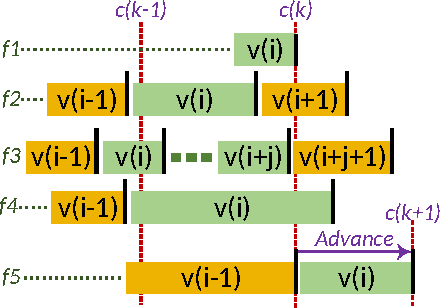
\includegraphics[width=\linewidth]{figs/scrr-packet-advance-finish.pdf}
    \vspace{-2mm}
    \caption{\small{\textit{Advancing the global clock in SCRR.}}}
	\label{fig:global-clock-finish}
    \end{subfigure}
    \begin{subfigure}[t]{.48\linewidth}
    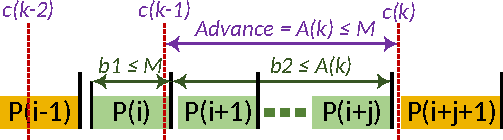
\includegraphics[width=\linewidth]{figs/scrr-packet-burst-finish.pdf}
    \vspace{-3mm}
    \caption{\small{\textit{Burstiness of SCRR.}}}
    \vspace{-3mm}
	\label{fig:burstiness-finish}
    \end{subfigure}
    \caption{\small{Analyzing SCRR with finish-time semantics.}}
 \vspace{-2mm}
\end{figure}



\subsection{Fairness of DRR with Variable Quanta}
\label{sub:variable-quanta}

We previously saw that the choice of the quanta in deficit round-robin impacts its
performance. A straw man argument might be to dynamically change DRR's quanta to enable it to adapt to changes in the traffic and environment. Alas, it is easy to show that this approach violates the fairness of the DRR scheduler.

A simple example illustrates the overall problem. Assume two
sub-queues are serviced by DRR. Assume that every time the first queue
is selected, the quanta is changed to a small value, and that every
time the second queue is selected, the quanta is changed to a large value. In this case, the second sub-queue is able to send much more data than the first sub-queue, hence causing unfairness.

A modified DRR could keep track of scheduling rounds, like what SCRR
does, and only allow quanta changes between rounds. We believe that
this change would make a DRR with dynamic quanta fair, but we have not
proven it in this study. The current Linux implementation of DRR in
the \textit{sch\_fq} module \cite{sch-fq} allocates quanta to
sub-queues when the deficit goes negative, so it is not strictly
aligned with scheduling rounds. Enforcing scheduling rounds in
\textit{sch\_fq} would most likely force non-trivial changes to the
code and make it less CPU efficient.